\documentclass[border=10pt]{standalone}
\usepackage{pgf,tikz,pgfplots}
\usetikzlibrary{quotes, angles}
\usetikzlibrary{positioning}
\usetikzlibrary{arrows.meta}
\usetikzlibrary{calc, shapes, automata, fit}
\usetikzlibrary{decorations.pathreplacing}
\tikzset{%
	% Specifications for style of nodes:
	base/.style = {rectangle, rounded corners, draw=black,
		%		minimum width=4cm, minimum height=1cm,
		inner sep=15pt,
		text centered, font=\sffamily}, 
	activityStarts/.style = {base, fill=blue!30},
	startstop/.style = {base, fill=red!30},
	activityRuns/.style = {base, fill=red!30},
	process/.style = {base, minimum width=2.5cm, fill=orange!15,
		font=\ttfamily},
	context/.style = {base, inner sep=5pt, align=justify, fill=blue!30}
}

\begin{document}
	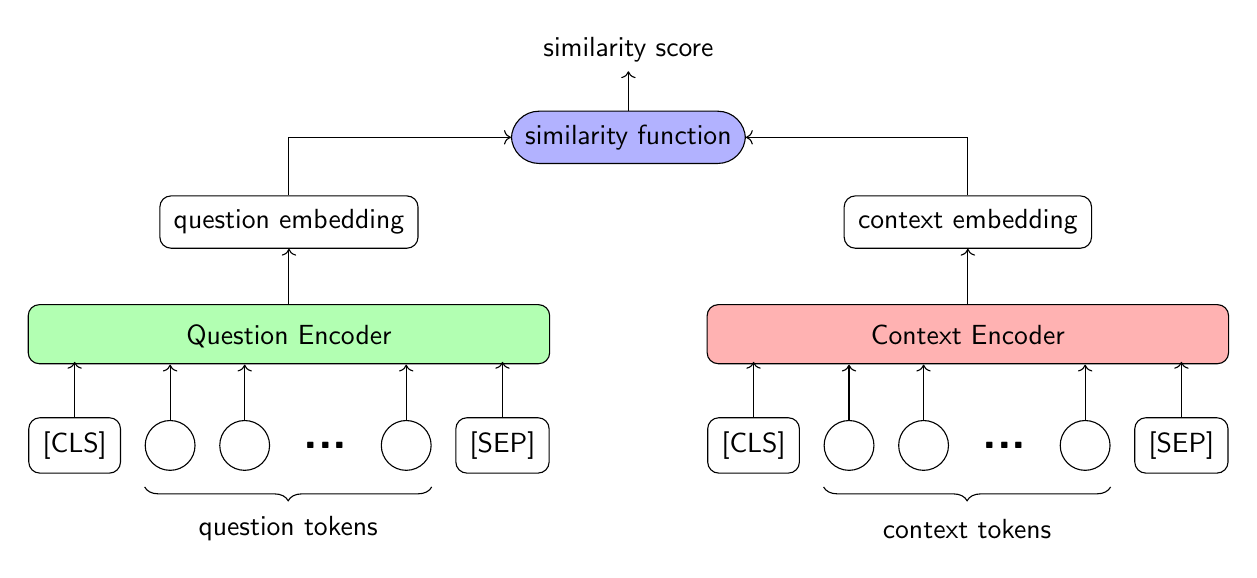
\begin{tikzpicture}[every node/.style={font=\sffamily}, align=center]
		\node [rounded corners, inner sep=5pt, draw=black] (qCLS) {[CLS]};
		\node [circle, draw=black, minimum size=18pt, right=.3cm of qCLS] (qTok1) {};
		\node [circle, draw=black, minimum size=18pt, right=.3cm of qTok1] (qTok2) {};
		\node [right=.3cm of qTok2, font=\fontsize{18pt}{\baselineskip}\selectfont\sffamily\bfseries] (qTokDots) {...};
		\node [circle, draw=black, minimum size=18pt, right=.3cm of qTokDots] (qTokLast) {};
		\node [rounded corners, draw=black, inner sep=5pt, minimum size=18pt, right=.3cm of qTokLast] (qSEP) {[SEP]};
		\path let
			\p1 = (qCLS.west),
			\p2 = (qCLS.north)
		in
			coordinate (qCLSAnchor) at (\x1, \y2);
		\path let
			\p1 = (qSEP.east),
			\p2 = (qSEP.north)
		in
			coordinate (qSEPAnchor) at (\x1, \y2);
		\coordinate[shift={(0., 20.pt)}] (qEncLL) at (qCLSAnchor);
		\coordinate[shift={(0., 40.pt)}] (qEncUR) at (qSEPAnchor);
		\node (qEnc) [fit={(qEncLL) (qEncUR)}, inner sep=0pt, draw=black, text height=0.5cm, text depth=0.25cm, fill=green!30, rounded corners] {Question Encoder};
		\draw[->] (qCLS.north) -- ++ (0., 20pt);
		\draw[->] (qTok1.north) -- ++ (0., 20pt);
		\draw[->] (qTok2.north) -- ++ (0., 20pt);
		\draw[->] (qTokLast.north) -- ++ (0., 20pt);
		\draw[->] (qSEP.north) -- ++ (0., 20pt);
		\coordinate[yshift=-15pt] (braceAnchorLeft) at (qTok1.west);
		\coordinate[yshift=-15pt] (braceAnchorRight) at (qTokLast.east); 
		\draw [decorate,decoration={brace,amplitude=5pt,mirror}] (braceAnchorLeft) -- (braceAnchorRight) node[midway, yshift=-15pt]{question tokens};
		\node[rounded corners, inner sep=5pt, draw=black, above=20.pt of qEnc] (qEmb) {question embedding};
		\draw[->] (qEnc) -- (qEmb);
		%% Context Encoder
		\node [rounded corners, inner sep=5pt, draw=black, right=2.cm of qSEP] (dCLS) {[CLS]};
		\node [circle, draw=black, minimum size=18pt, right=.3cm of dCLS] (dTok1) {};
		\node [circle, draw=black, minimum size=18pt, right=.3cm of dTok1] (dTok2) {};
		\node [right=.3cm of dTok2, font=\fontsize{18pt}{\baselineskip}\selectfont\sffamily\bfseries] (dTokDots) {...};
		\node [circle, draw=black, minimum size=18pt, right=.3cm of dTokDots] (dTokLast) {};
		\node [rounded corners, draw=black, inner sep=5pt, minimum size=18pt, right=.3cm of dTokLast] (dSEP) {[SEP]};
		\path let
			\p1 = (dCLS.west),
			\p2 = (dCLS.north)
		in
			coordinate (dCLSAnchor) at (\x1, \y2);
		\path let
			\p1 = (dSEP.east),
			\p2 = (dSEP.north)
		in
			coordinate (dSEPAnchor) at (\x1, \y2);
		\coordinate[shift={(0., 20.pt)}] (dEncLL) at (dCLSAnchor);
		\coordinate[shift={(0., 40.pt)}] (dEncUR) at (dSEPAnchor);
		\node (dEnc) [fit={(dEncLL) (dEncUR)}, inner sep=0pt, draw=black, text height=0.5cm, text depth=0.25cm, fill=red!30, rounded corners] {Context Encoder};
		\draw[->] (dCLS.north) -- ++ (0., 20pt);
		\draw[->] (dTok1.north) -- ++ (0., 20pt);
		\draw[->] (dTok2.north) -- ++ (0., 20pt);
		\draw[->] (dTokLast.north) -- ++ (0., 20pt);
		\draw[->] (dSEP.north) -- ++ (0., 20pt);
		\coordinate[yshift=-15pt] (DbraceAnchorLeft) at (dTok1.west);
		\coordinate[yshift=-15pt] (DbraceAnchorRight) at (dTokLast.east); 
		\draw [decorate,decoration={brace,amplitude=5pt,mirror}] (DbraceAnchorLeft) -- (DbraceAnchorRight) node[midway, yshift=-15pt]{context tokens};
		\node[rounded corners, inner sep=5pt, draw=black, above=20.pt of dEnc] (dEmb) {context embedding};
		\draw[->] (dEnc) -- (dEmb);
		%% Similarity func
		\path let
			\p1 = (qEnc.east),
			\p2 = (dEnc.west)
		in
			coordinate (center) at (\x1 / 2 + \x2 / 2, \y1);
		\node[yshift=2.5cm, rounded corners=10, draw=black, inner sep=5pt, fill=blue!30] (simFunc)  at (center) {similarity function};
		%% path
		\draw [->] (qEmb) |- (simFunc);
		\draw [->] (dEmb) |- (simFunc);
		\node [above=0.5cm of simFunc] (simScore) {similarity score};
		\draw[->] (simFunc) -- (simScore);
	\end{tikzpicture}
\end{document}